\chapter{Time Integration}
In this chapter, the evolution of an equation will be analyzed by looking at the time evolutions of two Partial Differential Equations (PDEs), namely the Advection Equation (Equation \ref{adveq}) and the Wave Equation (Equation \ref{waveeq}).
\begin{equation} \label{adveq}
\begin{align}
  &u_t + cu_x = 0, \qquad c \in \mathbb{R} \\ 
  &u(x,0) = u_0(x)
\end{align}
\end{equation}
\begin{equation} \label{waveeq}
\begin{align}
  &u_{tt} - c^2u_{xx} = 0, \qquad c \in \mathbb{R} \\ 
  &u(x,0) = u_0(x), \qquad u_t(x,0) = p_0(x)
\end{align}
\end{equation}
%%%%%%%%%%%%%%%%%%%%%%%%%%%%%%%%%%%%%%%%%%%%%%%%%%%%%%%%%%%%%%%%%%%%%
\section{Characteristic Structure}
Characteristics are a way of simplifying an equation by changing the coordinates in which the PDE is calculated. It also shows how the information of the PDE propagates with time.
%-------------------------------------------------------------------
\subsection{Advection Equation}
The Advection Equation is a first order PDE (meaning the highest order derivative is in the first order). This means we need only specify one characteristic, $p$. Where $x = x(p)$ and $t = t(p)$ therefore $u = u(x,t) = u(x(p),t(p)) = u(p)$.
\linebreak
\linebreak
By the method of characteristics we can determine that the characteristic equations for the Advection equation are
\begin{equation}
\frac{dx}{dp} = c, \qquad \frac{dt}{dp} = 1, \qquad \frac{du}{dp} = 0
\end{equation}
which are then integrated to give
\begin{equation}
  x = cp + C_1, \qquad t = p + C_2, \qquad u = C_3
\end{equation}
By setting $p=0$ at $t=0$, $C_2$ is set to 0 and $t=p$ everywhere. Setting $x=p$ along $u_0(x)$ gives us 
\begin{equation}
x=cp+q \qquad \text{and} \qquad u=u_0(q).
\end{equation}
\linebreak
\linebreak
$x=cp+q$ and $t=p$ can be used to give us the characteristic coordinate 
\begin{equation}
q=x-ct
\end{equation}
which is a line with a slope of $c$ in the $(x,t)-plane$. Substituting this into $u_0$ gives us
\begin{equation}
  u = u_0(x - ct)
\end{equation}
%--------------------------------------------------------------------
\subsection{Wave Equation}
The Wave Equation is a second order PDE, therefore it has two characteristics. $p$ and
$q$.By reducing the equation to its canonical form, $u_{pq} = 0$. In this we see that 
\begin{equation} \label{wavecoords}
p = x-ct \qquad \text{and} \qquad q = x + ct
\end{equation}
Since $u_{pq} = u_{qp} = 0$ then it follows that $u_p = P(p)$. Let $F(p)$ be an anti-derivative of $P$ therefore $\frac{dF}{dp}(p) = P(p)$ and therefore 
\begin{equation}
\frac{\partial}{\partial p}(u - F(p)) = 0
\end{equation}
by integrating both sides, it then follows that
\begin{equation}
u - F(p) = G(q)
\end{equation}
and therefore by rearranging and substituting Equation \ref{wavecoords}, we get
\begin{equation}
u(x,t) = F(x-ct) + G(x+ct)
\end{equation}
By analyzing this solution and comparing it to that of the Advection Equation, we see that we in fact get two characteristic coordinates which are lines with slopes of $\pm c$.
%-------------------------------------------------------------------
\subsection{Spacing}
Along with finding the characteristics comes the trouble of determining the spacing for the spacial and time axis when plotting. The spacial spacing will be denoted by $h$ and time by $k$. If $h<k$ then the data needed to determine the value of the function at a given point in space and time will require data outside of the bounds of the stencil, conversely if $h>k$ then data between two spacial points is needed to calculate the next value, but this can be interpolated at the cost of calculation time and may yield a higher accuracy. The standard is to set $h=k$ so that the stencil exactly fits the data needed to calculate the next point and every point being used need not be interpolated as it falls on an existing point in the spacing. This can be seen in the figures in Figure \ref{fig:advcoordimg} for the Advection Equation and in Figure \ref{fig:wavecoordimg} for the Wave Equation.
%----------------------------------------------------------------------
\begin{figure}[H]
\centering
\begin{subfigure}[b]{0.3\textwidth}
  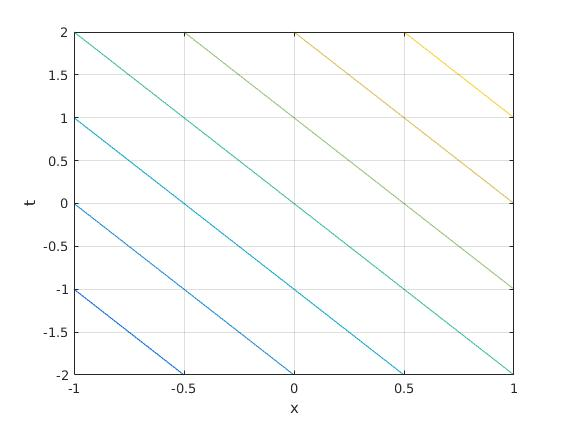
\includegraphics[width=\textwidth]{Images/advection_h<k.jpg}
  \caption{$h<k$}
  \label{fig:aci1}
\end{subfigure}
\hfill
\begin{subfigure}[b]{0.3\textwidth}
  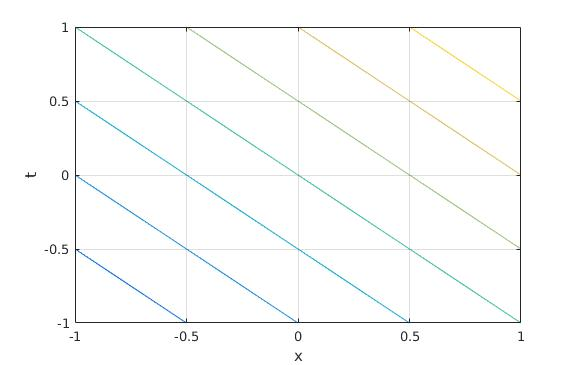
\includegraphics[width=\textwidth]{Images/advection_h=k.jpg}
  \caption{$h=k$}
  \label{fig:aci2}
\end{subfigure}
\hfill
\begin{subfigure}[b]{0.3\textwidth}
  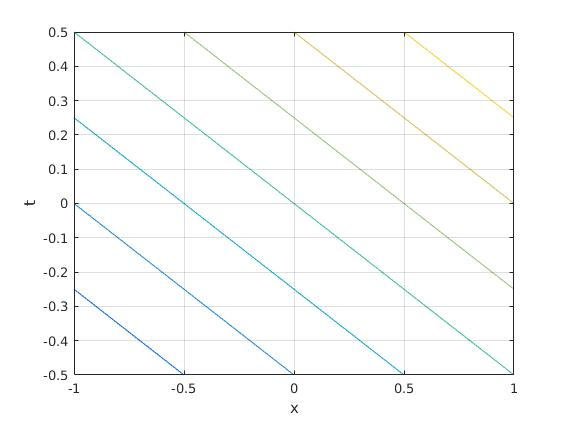
\includegraphics[width=\textwidth]{Images/advection_h>k.jpg}
  \caption{$h>k$}
  \label{fig:aci3}
\end{subfigure}
\caption{Advection characteristic}
\label{fig:advcoordimg}
\end{figure}
%----------------------------------------------------------------------
\begin{figure}[H]
\centering
\begin{subfigure}[b]{0.3\textwidth}
  \centering
  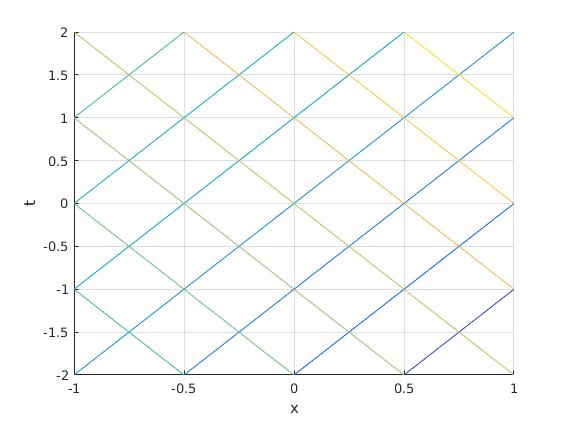
\includegraphics[width=\textwidth]{Images/wave_h<k.jpg}
  \caption{$h<k$}
  \label{fig:wci1}
\end{subfigure}
\hfill
\begin{subfigure}[b]{0.3\textwidth}
  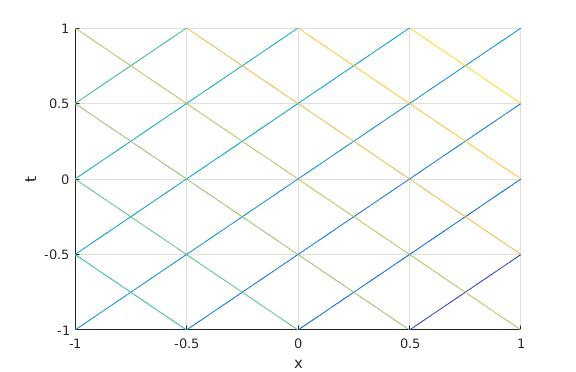
\includegraphics[width=\textwidth]{Images/wave_h=k.jpg}
  \caption{$h=k$}
  \label{fig:wci2}
\end{subfigure}
\hfill
\begin{subfigure}[b]{0.3\textwidth}
  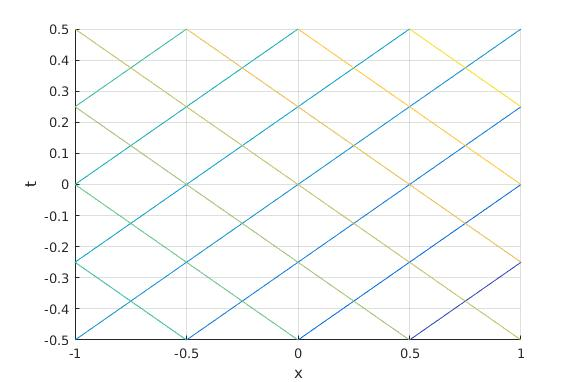
\includegraphics[width=\textwidth]{Images/wave_h>k.jpg}
  \caption{$h>k$}
  \label{fig:wci3}
\end{subfigure}
\caption{Wave Equation Charactersitics}
\label{fig:wavecoordimg}
\end{figure}
%%%%%%%%%%%%%%%%%%%%%%%%%%%%%%%%%%%%%%%%%%%%%%%%%%%%%%%%%%%%%%%%%%%%%%%
\section{Discretization}
Using the FDM discussed in Chapter 2 we will confirm the validity of three approximations of the advection equation, the Centered Euler, Leapfrog, and Upwind Euler methods, and the Leapfrog approximation of the wave equation.
%-----------------------------------------------------------------
\subsection{Advection Equation}
The advection equation can be approximated with the function $v$ where
\begin{equation}
v_i^j = u(x_i,t_j)
\end{equation}
by using the standard FDM we get the partial derivatives
\begin{equation}\label{advfdm}
\begin{align}
    \partial_xv_i^j &= \frac{v_{i+1}^j - v_{i-1}^j}{2h} + O(h^2) \\
    \partial_tv_i^j &= \frac{v_i^{j+1} - v_i^{j-1}}{2k} + O(k^2)
\end{align}
\end{equation}
%-----------------------------------------------------------------
\subsubsection{Leapfrog}
Substituting Equation \ref{advfdm} into the advection equation we get
\begin{equation}
  \partial_tv_i^j + c\partial_xv_i^j = 0
\end{equation}
however, $v_i^{j+1}$ is unknown. So we rearrange the equation to solve for $v_i^{j+1}$ to get
\begin{equation}
\begin{align}
    v_i^{j+1} &= v_i^{j-1} - 2ck\partial_xv_i^j \\
	      &= v_i^{j-1} - c\frac{k}{h}(v_{i+1}^j - v_{i-1}^j) + O(h^2k^2)
\end{align}
\end{equation}
This is known as the ``Leapfrog'' method as it requires $v_i^{j-1}$ in order to calculate $v_i^{j+1}$ This can be somewhat problematic with the initial data as $v_i^0=u_0$ and $v_i^2$ onwards can be calculated this way but $v_i^1$ cannot be found by this method. Another problem concerining this method is the decoupling of odd and even points as all even points rely soley on the odd points of the previous time step and alternately for the odd points.
%-----------------------------------------------------------------
\subsubsection{Centered Euler}
The Centred Euler method seeks to circumvent this problem by setting
\begin{equation}
\partial_tv_i^j = \frac{v_i^{j+1} - v_i^j}{k} + O(k) 
\end{equation}
substituting this into the advection equation and rearranging to solve for $v_i^{j+1}$ gives
\begin{equation}
\begin{align}
    v_i^{j+1} &= v_i^j - ck\partial_xv_i^j \\
	      &= v_i^j - c\frac{k}{2h}(v_{i+1}^j - v_{i-1}^j) + O(kh^2)
\end{align}
\end{equation}
This method uses a one-sided time step to calculate the next step. This makes it unconditionally unstable and over time it varies wildly from the actual data. Due to the error being relatively low for the first step, it is generally used to initialise the Leapfrog method.
%-----------------------------------------------------------------
\subsubsection{Upwind Euler}
By setting
\begin{equation}
\begin{align}
    \partial_xv_i^j &= \frac{v_{i+1}^j - v_i^j}{h} + O(h) \\
    \partial_tv_i^j &= \frac{v_i^{j+1} - v_i^j}{k} + O(k)
\end{align}
\end{equation}
we get
\begin{equation}
\begin{align}
    v_i^{j+1} &= v_i^j - ck\partial_xv_i^j \\
	      &= v_i^j - c\frac{k}{h}(v_{i+1}^j - v_i^j) + O(kh)
\end{align}
\end{equation}
This is arguably the best method to calculate the advection equation as it uses a biased stencil to propel the data from $u_0$ along the $t$ and $x$ axis, much like the advection equation itself.
%-----------------------------------------------------------------
\subsection{Wave Equation}
Using the second order, second derivative FDM on $u$ with $v_i^j = u(x_i,t_j)$ we get
\begin{equation}
\begin{align}
    \partial_{xx}v_i^j &= \frac{v_{i+1}^j - 2v_i^j + v_{i-1}^j}{h^2} + O(h^2) \\
    \partial_{tt}v_i^j &= \frac{v_i^{j+1} - 2v_i^j + v_i^{j-1}}{k^2} + O(k^2)
\end{align}
\end{equation}
Substituting this into the wave equation we get
\begin{equation}
  \partial_{tt}v_i^j - c^2\partial_{xx}v_i^j = 0
\end{equation}
As with the advection equation, $v_i^{j+1}$ is unknown. reaaringing to solve for this, we get
\begin{equation}
  v_i^{j+1} = 2v_i^j - v_i^{j+1} + c^2\frac{k^2}{h^2}(v_{i+1}^j - 2v_i^j + v_{i-1}^j) + O(h^2k^2)
\end{equation}
This is a Leapfrog method approximation similar to that of the advection equation, it however does not have the decoupling of points as this stencil uses three points from the previous time step as opposed to the two used by the advection equation. This method also has the problem of $v_i^1$ being needed as initial data, this can usually be solved by calculating the row by hand and then feeding it into the system as initial data.
%%%%%%%%%%%%%%%%%%%%%%%%%%%%%%%%%%%%%%%%%%%%%%%%%%%%%%%%%%%%%%%%%%%%%%%%%%%%%%%%
\section{Implimentation}
The initial equation
\begin{equation}
  u(x,0) = e^{-x^2}
\end{equation}
was calculated on the interval $-10<x<10$ and $0<t<20$ with $100$ and $1000$ data points and compared to the exact solution, the L2-norm of the error was also analysed. For each solution the ghost points were a periodic extension of the previous steps data. The results were as follows
%-------------------------------------------------------------------------------
\subsection{Centered Euler Advection Equation}
The exact solution to the equation is
\begin{equation}
u(x,t) = e^{-(x-t)^2}
\end{equation}
The wild variance of the Centered Euler method can be seen after only two seconds in Figure \ref{center_euler_adv}. The L2-norm of the error exponentially increases over time as seen in Figure \ref{center_euler_adv_l2}.
%-------------------------------------------------------------------------------
\begin{figure}[H] 
 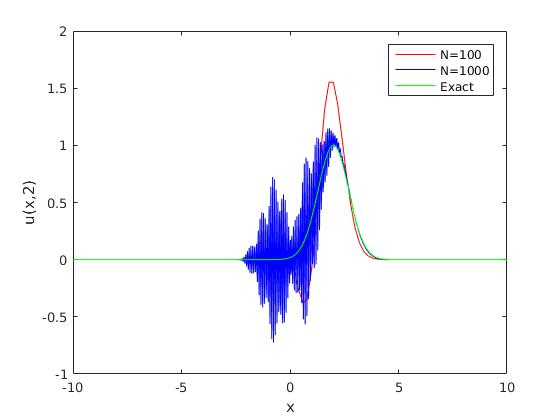
\includegraphics[scale=0.5]{Images/center_euler_adv.jpg}
 \caption{Advection Equation and Approximations after 2 seconds}
 \label{center_euler_adv}
\end{figure}
\begin{figure}[H] 
 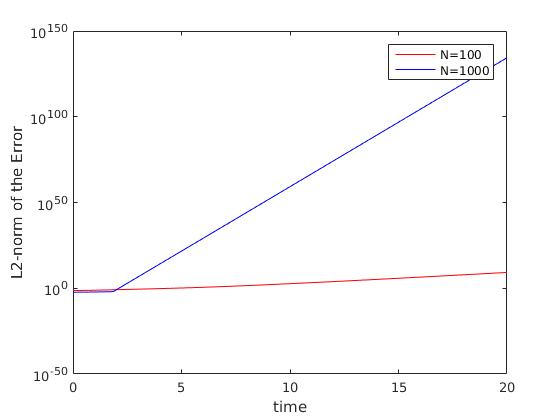
\includegraphics[scale=0.5]{Images/center_euler_adv_l2.jpg}
 \caption{Change in L2-norm over time of Centered Euler Evolution}
 \label{center_euler_adv_l2}
\end{figure}
%-------------------------------------------------------------------------------
\subsection{Leapfrog Advection Equation}
The L2-norm of the error as seen in Figure \ref{leapfrog_adv_l2} is due to the ghost points of the approximation being treated as a periodic extension of the function causing the function to be repeated every 20 time steps, the start of this can be seen in Figure \ref{leapfrog_adv}, which shows the functions after nine time steps.
%-------------------------------------------------------------------------------
\begin{figure}[H] 
 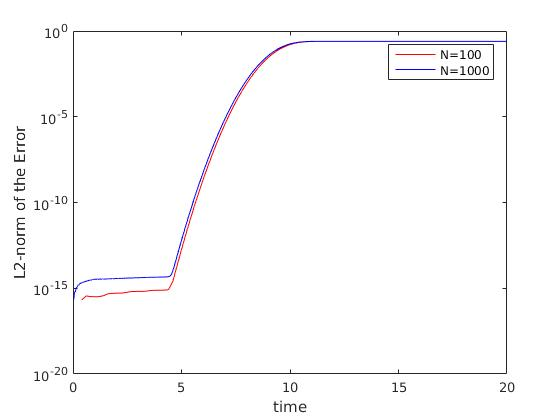
\includegraphics[scale=0.5]{Images/leapfrog_adv_l2.jpg}
 \caption{Change in L2-norm over time of Leapfrog Evolution}
 \label{leapfrog_adv_l2}
\end{figure}
\begin{figure}[H]
 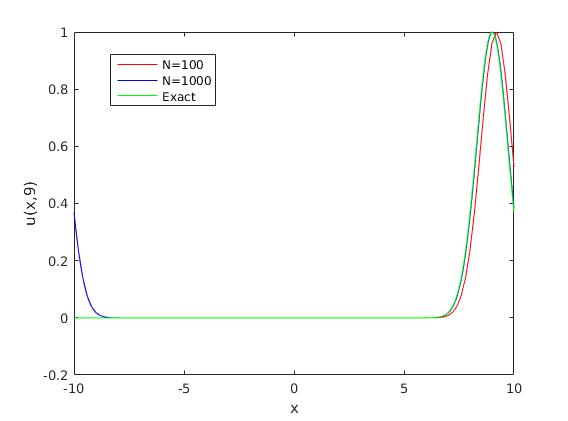
\includegraphics[scale=0.5]{Images/leapfrog_adv.jpg}
 \caption{Advection Equation and Approximations after 9 seconds}
 \label{leapfrog_adv}
\end{figure}
%-------------------------------------------------------------------------------
\subsection{Leapfrog Wave Equation}
The exact solution to the equation is
\begin{equation}
u(x,t) = \frac{1}{2}(e^{-(x-t)^2} + e^{-(x+t)^2})
\end{equation}
Figure \ref{leapfrog_wave} shows how this approximation suffers from the same problem as the leapfrog advection approximation since it too has ghost points which see the function as a periodic extension and leads to the same problem of steps in the L2-norm of the error, shown in Figure \ref{leapfrog_wave_l2}. Adjusting the size of the time steps by making $k=0.5h$ leads to a minor reduction in the L2-norm of the error, as seen in Figure \ref{leapfrog_wave_l2_halfk}, however with the large steps due to the periodic extension this is almost unnoticeable, if the time step is doubled to $k=2h$ then the error increases exponentially over time after a relatively short period of time, seen in Figure \ref{leapfrog_wave_l2_2k}.
%-------------------------------------------------------------------------------
\begin{figure}[H] 
 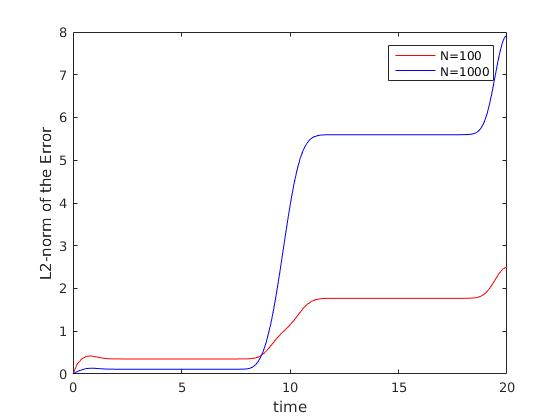
\includegraphics[scale=0.5]{Images/leapfrog_wave_l2.jpg}
 \caption{Change in L2-norm over time of Leapfrog Evolution with $k = h$}
 \label{leapfrog_wave_l2}
\end{figure}
\begin{figure}[H] 
 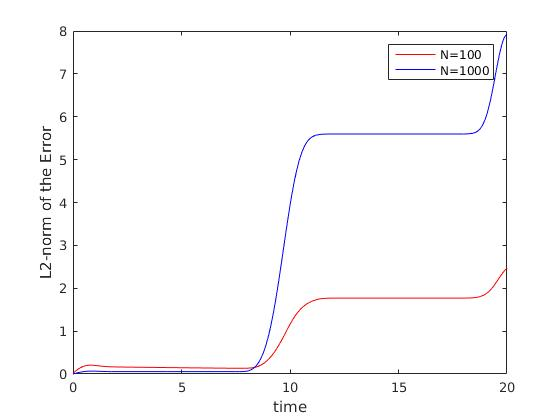
\includegraphics[scale=0.5]{Images/leapfrog_wave_l2_halfk.jpg}
 \caption{Change in L2-norm over time of Leapfrog Evolution with $k = 0.5h$}
 \label{leapfrog_wave_l2_halfk}
\end{figure}
\begin{figure}[H] 
 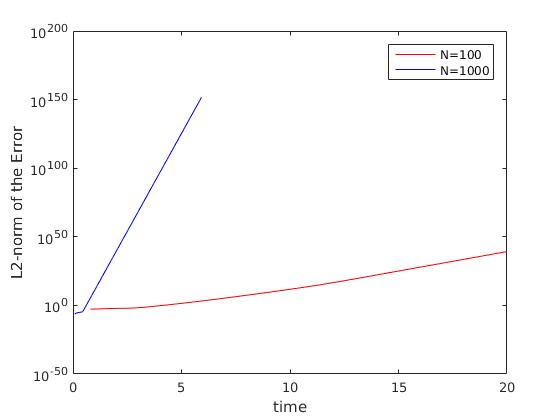
\includegraphics[scale=0.5]{Images/leapfrog_wave_l2_2k.jpg}
 \caption{Change in L2-norm over time of Leapfrog Evolution with $k = 2h$}
 \label{leapfrog_wave_l2_2k}
\end{figure}
\begin{figure}[H] 
 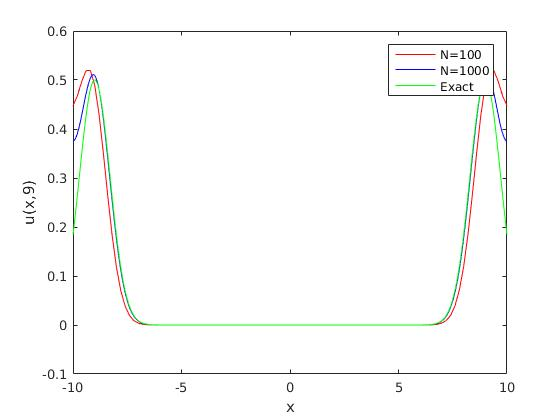
\includegraphics[scale=0.5]{Images/leapfrog_wave.jpg}
 \caption{Wave Equation and Approximations after 9 seconds}
 \label{leapfrog_wave}
\end{figure}
%%%%%%%%%%%%%%%%%%%%%%%%%%%%%%%%%%%%%%%%%%%%%%%%%%%%%%%%%%%%%%%%%%%%%%%%%%%%%%%%